\documentclass[UKenglish]{ifimaster}
\usepackage[latin1]{inputenc}
\usepackage[T1]{fontenc,url}
\urlstyle{sf}
\usepackage{babel,textcomp,csquotes,duomasterforside,varioref,graphicx}
\usepackage[backend=biber,style=numeric-comp]{biblatex}

\title{The title of my thesis}
\subtitle{Any short subtitle}
\author{Lucas Charpentier}

\bibliography{mybib}

\graphicspath{ {images/} }

\begin{document}
\duoforside[program={Computational Science},
    option={Imaging and Biomedical Computing},
    dept={Departement of Informatics \and Departement of Physics},
    long
    ]
\frontmatter{}
\maketitle{}

\chapter*{Abstract}
\tableofcontents{}
\listoffigures{}
\listoftables{}

\chapter*{Preface}

\mainmatter{}

\chapter{Introduction}
    \section{Background and Motivation}
    
    
    \section{Problem Statement}


    \section{Thesis Outline}


\chapter{Planning the project}
    \section{Machine Learning}
        \subsection{Supervised Learning}
        
        
        \subsection{Unsupervised Learning}

    
    \section{Artificial Neural Networks}
        \subsection{Perceptron}


        \subsection{Multilayer Perceptron}


        \subsection{Training a Neural Network}

    
    \section{Convolutional Neural Network}
        \subsection{Convolutional Layers}


        \subsection{Pooling Layers}

    
    \section{Neural Network Training Optimization}
        \subsection{Weight Initialization}


        \subsection{Training Batch Size}


        \subsection{Dropout}


    \section{Network Pruning}

    
    \section{Datasets}
        \subsection{MNIST}


        \subsection{Fashion MNIST}


        \subsection{CIFAR-10}


    \section{Architectures}
        \subsection{VGG-16}

\chapter{Single Layer ANN}
    \section{Pruning Nodes at Random}
        \subsection{MNIST}
            Artificial Neural Network with single hidden layer of 128 nodes, using ADAM as optimizer with a learning rate of 0.001 trained on 5 epochs, batch size of 32.
            Final Accuracy and Loss on test set are:
            Loss: 0.0734
            Accuracy: 0.9770
            \begin{table}[h!]
                \centering
                \begin{tabular}{c | c c c c c c c}
                    & \multicolumn{7}{c}{\textbf{Number of Nodes}} \\
                    \cline{2-8}
                    & 1 & 2 & 4 & 8 & 16 & 32 & 64 \\
                    \hline
                    \textbf{Mean} & 0.9765 & 0.9760 & 0.9750 & 0.9724 & 0.9658 & 0.9464 & 0.8555 \\
                    \textbf{$\sigma$} & 0.0007 & 0.0010 & 0.0015 & 0.0027 & 0.0053 & 0.0122 & 0.0394 \\
                    \textbf{min} & 0.9740 & 0.9660 & 0.9635 & 0.9494 & 0.9337 & 0.8688 & 0.6598 \\
                    \textbf{25\%} & 0.9762 & 0.9756 & 0.9742 & 0.9710 & 0.9632 & 0.9410 & 0.8331 \\
                    \textbf{50\%} & 0.9767 & 0.9762 & 0.9753 & 0.9728 & 0.9669 & 0.9489 & 0.8616 \\
                    \textbf{75\%} & 0.9770 & 0.9767 & 0.9760 & 0.9742 & 0.9695 & 0.9543 & 0.8837 \\
                    \textbf{max} & 0.9778 & 0.9780 & 0.9779 & 0.9769 & 0.9769 & 0.9685 & 0.9334 \\
                    
                \end{tabular}
                \caption[Short]{Long}
            \end{table}

            Trial text

            \begin{figure}[h!]\centering
                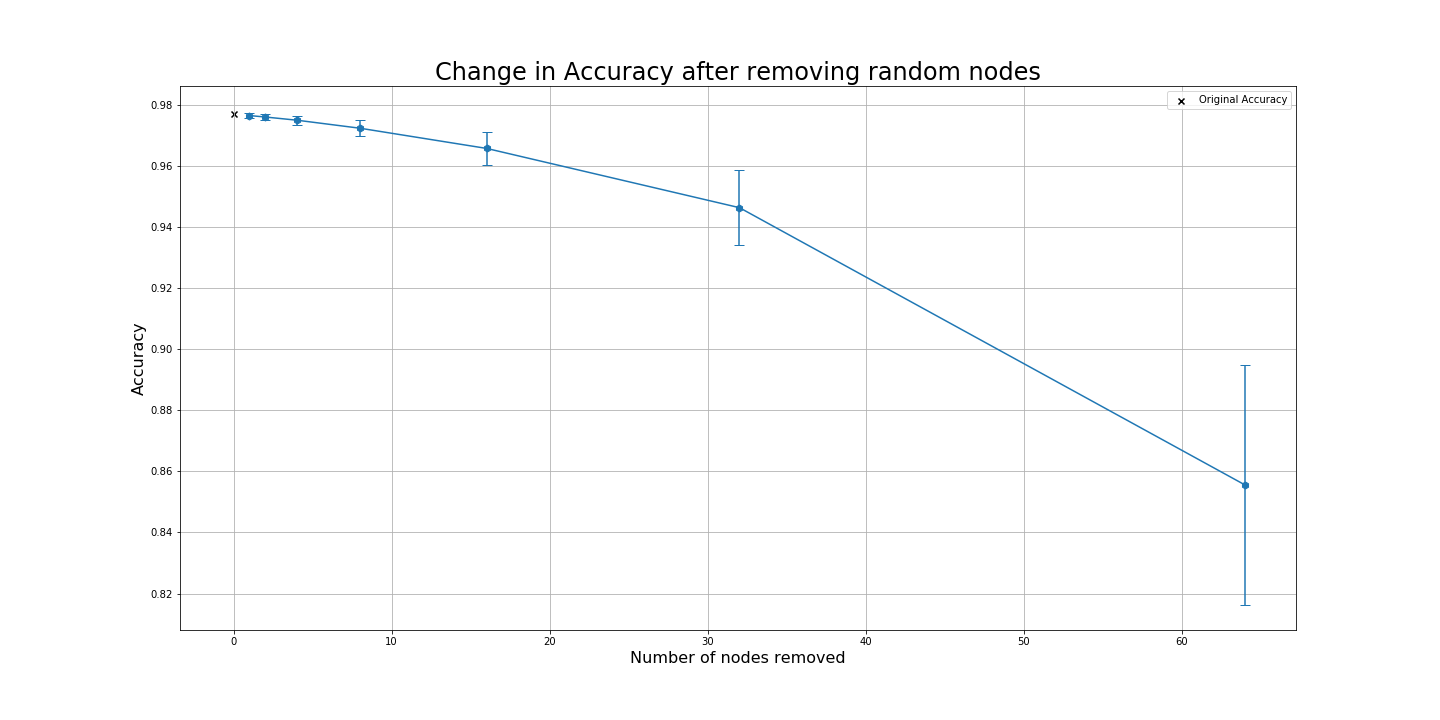
\includegraphics[width=\textwidth]{Accuracy_change_random_removal_mnist.png}
                \caption[Short title]{Testing}
                \label{fig:acc_rn_mnist}
            \end{figure}

            Trial text

            \begin{table}[h!]
                \centering
                \begin{tabular}{c | c c c c c c c}
                    & \multicolumn{7}{c}{\textbf{Number of Nodes}} \\
                    \cline{2-8}
                    & 1 & 2 & 4 & 8 & 16 & 32 & 64 \\
                    \hline
                    \textbf{Mean} & 0.0751 & 0.0767 & 0.0801 & 0.0885 & 0.1090 & 0.1680 & 0.4298 \\
                    \textbf{$\sigma$} & 0.0023 & 0.0032 & 0.0047 & 0.0083 & 0.0157 & 0.0338 & 0.0989 \\
                    \textbf{min} & 0.0720 & 0.0714 & 0.0710 & 0.0735 & 0.0791 & 0.1006 & 0.2311 \\
                    \textbf{25\%} & 0.07 & 0. & 0.9742 & 0.9710 & 0.9632 & 0.9410 & 0.8331 \\
                    \textbf{50\%} & 0.9767 & 0.9762 & 0.9753 & 0.9728 & 0.9669 & 0.9489 & 0.8616 \\
                    \textbf{75\%} & 0.9770 & 0.9767 & 0.9760 & 0.9742 & 0.9695 & 0.9543 & 0.8837 \\
                    \textbf{max} & 0.9778 & 0.9780 & 0.9779 & 0.9769 & 0.9769 & 0.9685 & 0.9334 \\
                    
                \end{tabular}
                \caption[Short]{Long}
            \end{table}

            Trial text

            \begin{figure}[h!]\centering
                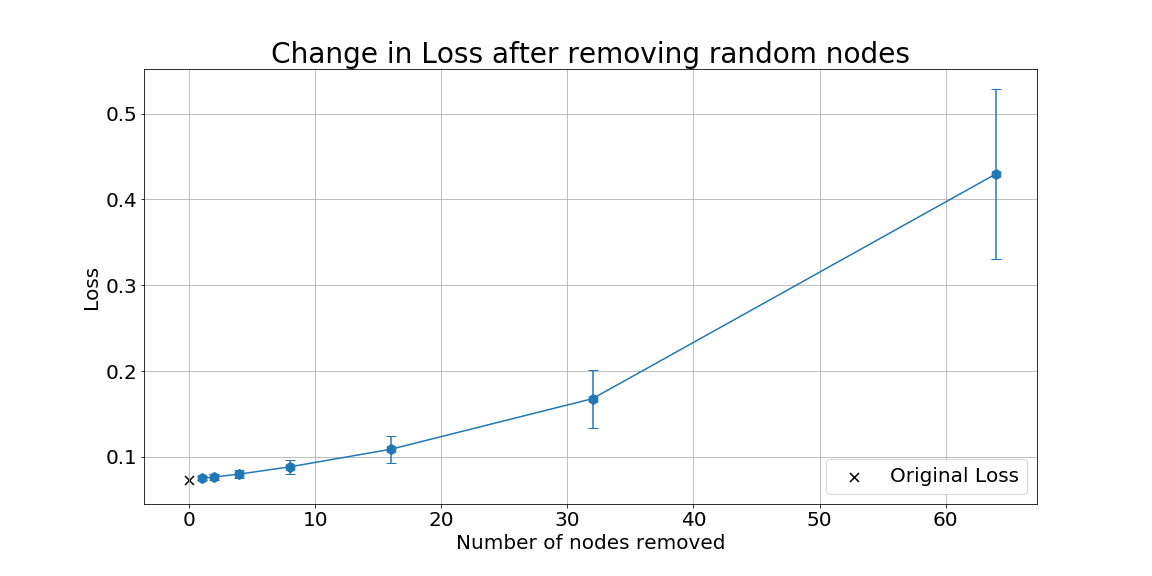
\includegraphics[width=\textwidth]{Loss_change_random_removal_mnist.png}
                \caption[Short title]{Testing}
                \label{fig:loss_rn_mnist}
            \end{figure}

            Trial text

            \begin{table}[h!]
                \centering
                \begin{tabular}{c | c c c c c c c}
                    & \multicolumn{7}{c}{\textbf{Number of Nodes}} \\
                    \cline{2-8}
                    & 1 & 2 & 4 & 8 & 16 & 32 & 64 \\
                    \hline
                    \textbf{Mean} & 0.0751 & 0.0767 & 0.0801 & 0.0885 & 0.1090 & 0.1680 & 0.4298 \\
                    \textbf{$\sigma$} & 0.0023 & 0.0032 & 0.0047 & 0.0083 & 0.0157 & 0.0338 & 0.0989 \\
                    \textbf{min} & 0.0720 & 0.0714 & 0.0710 & 0.0735 & 0.0791 & 0.1006 & 0.2311 \\
                    \textbf{25\%} & 0. & 0.9756 & 0.9742 & 0.9710 & 0.9632 & 0.9410 & 0.8331 \\
                    \textbf{50\%} & 0.9767 & 0.9762 & 0.9753 & 0.9728 & 0.9669 & 0.9489 & 0.8616 \\
                    \textbf{75\%} & 0.9770 & 0.9767 & 0.9760 & 0.9742 & 0.9695 & 0.9543 & 0.8837 \\
                    \textbf{max} & 0.9778 & 0.9780 & 0.9779 & 0.9769 & 0.9769 & 0.9685 & 0.9334 \\
                    
                \end{tabular}
                \caption[Short]{Long}
            \end{table}

            Trial text

            \begin{figure}[h!]\centering
                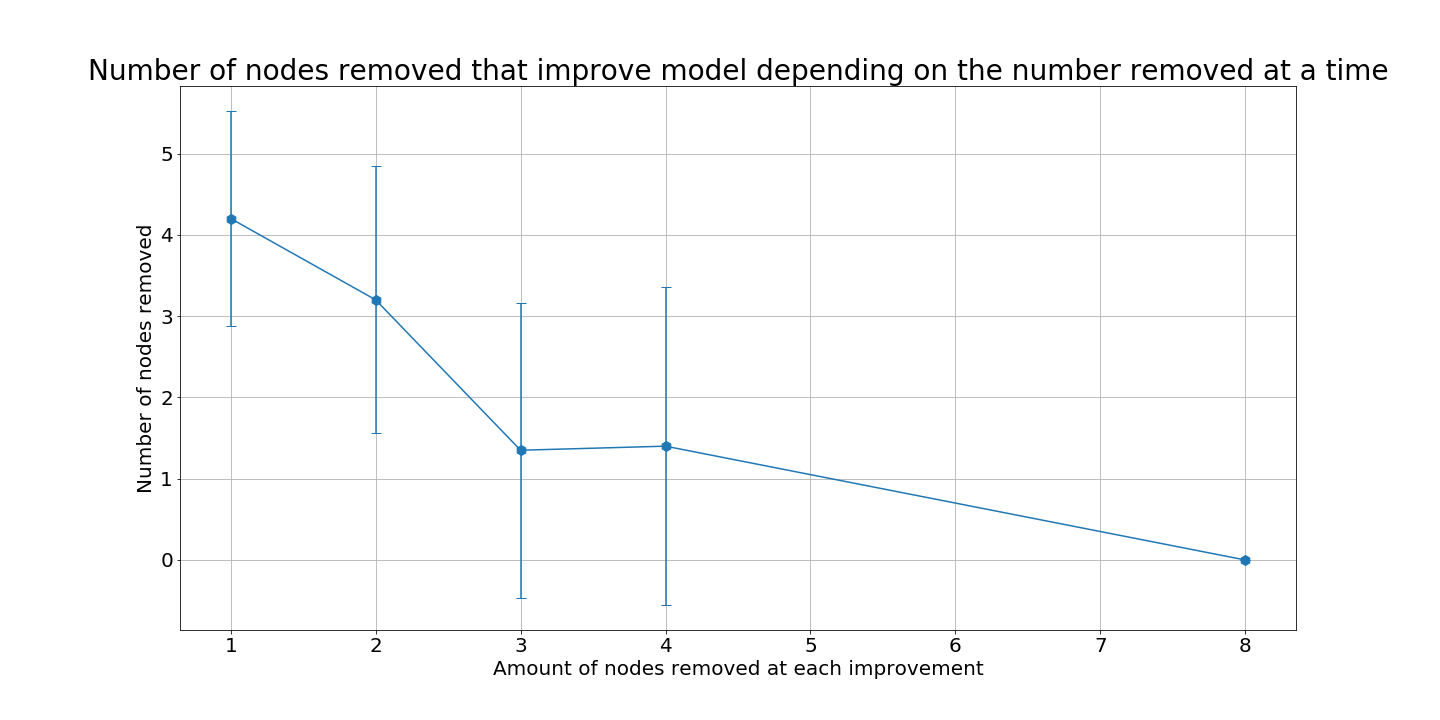
\includegraphics[width=\textwidth]{Num_rem_vs_size_removed_mnist.png}
                \caption[Short title]{Testing}
                \label{fig:num_rem_rn_imp_mnist}
            \end{figure}

            Trial text

            \begin{figure}[h!]\centering
                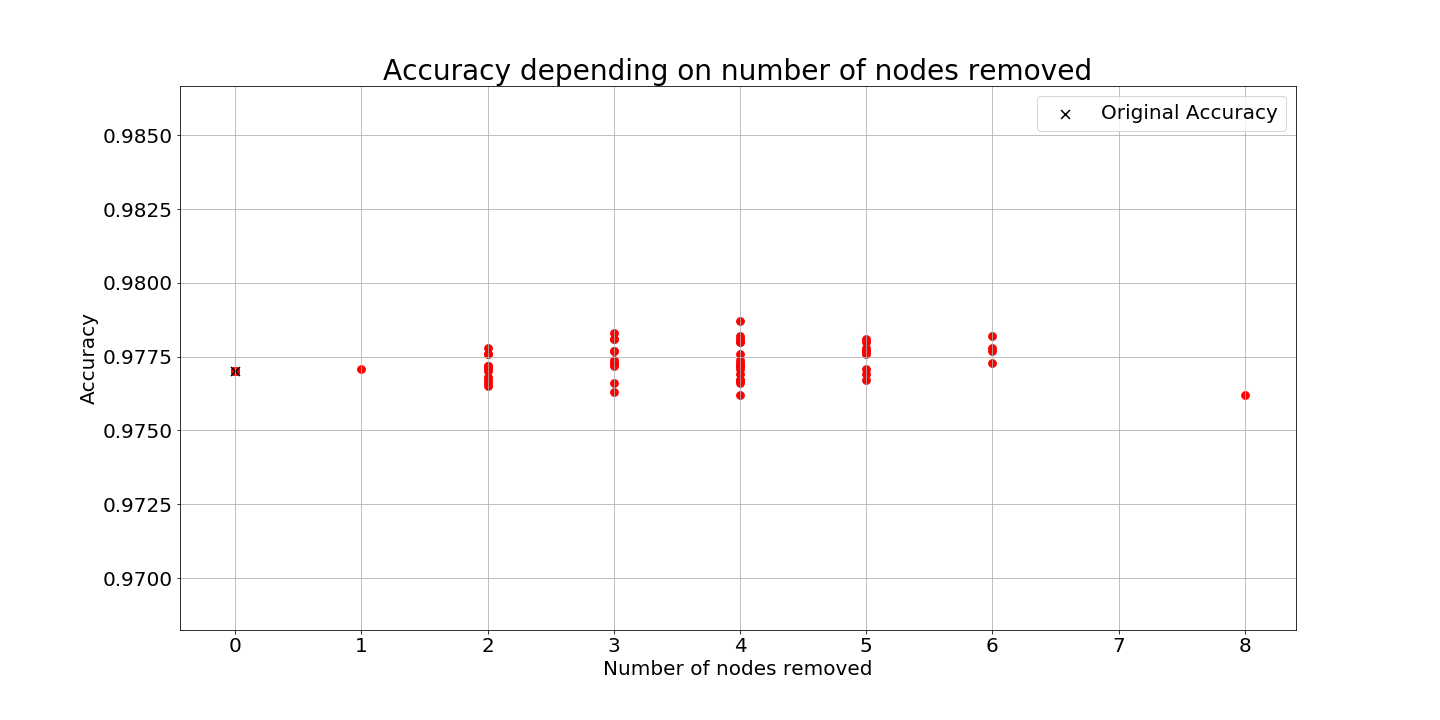
\includegraphics[width=\textwidth]{Accuracy_vs_nodes_removed_mnist.png}
                \caption[Short title]{Testing}
                \label{fig:acc_rn_imp_mnist}
            \end{figure}

            Trial text

            \begin{figure}[h!]\centering
                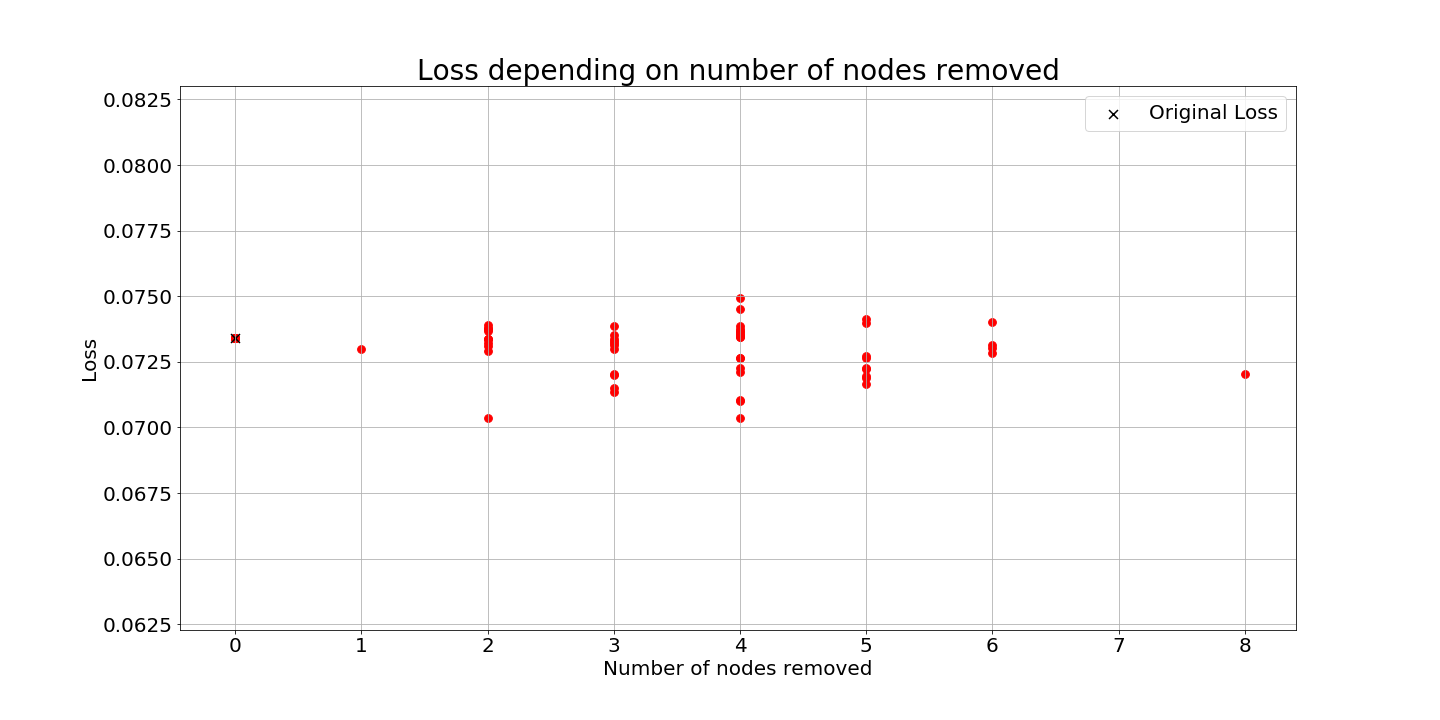
\includegraphics[width=\textwidth]{Loss_vs_nodes_removed_mnist.png}
                \caption[Short title]{Testing}
                \label{fig:loss_rn_imp_mnist}
            \end{figure}

            Trial text

        \subsection{Fashion MNIST}

            Trial text

            \begin{table}[h!]
                \centering
                \begin{tabular}{c | c c c c c c c}
                    & \multicolumn{7}{c}{\textbf{Number of Nodes}} \\
                    \cline{2-8}
                    & 1 & 2 & 4 & 8 & 16 & 32 & 64 \\
                    \hline
                    \textbf{Mean} & 0.9765 & 0.9760 & 0.9750 & 0.9724 & 0.9658 & 0.9464 & 0.8555 \\
                    \textbf{$\sigma$} & 0.0007 & 0.0010 & 0.0015 & 0.0027 & 0.0053 & 0.0122 & 0.0394 \\
                    \textbf{min} & 0.9740 & 0.9660 & 0.9635 & 0.9494 & 0.9337 & 0.8688 & 0.6598 \\
                    \textbf{25\%} & 0.9762 & 0.9756 & 0.9742 & 0.9710 & 0.9632 & 0.9410 & 0.8331 \\
                    \textbf{50\%} & 0.9767 & 0.9762 & 0.9753 & 0.9728 & 0.9669 & 0.9489 & 0.8616 \\
                    \textbf{75\%} & 0.9770 & 0.9767 & 0.9760 & 0.9742 & 0.9695 & 0.9543 & 0.8837 \\
                    \textbf{max} & 0.9778 & 0.9780 & 0.9779 & 0.9769 & 0.9769 & 0.9685 & 0.9334 \\
                    
                \end{tabular}
                \caption[Short]{Long}
            \end{table}

            Trial text

            \begin{figure}[h!]\centering
                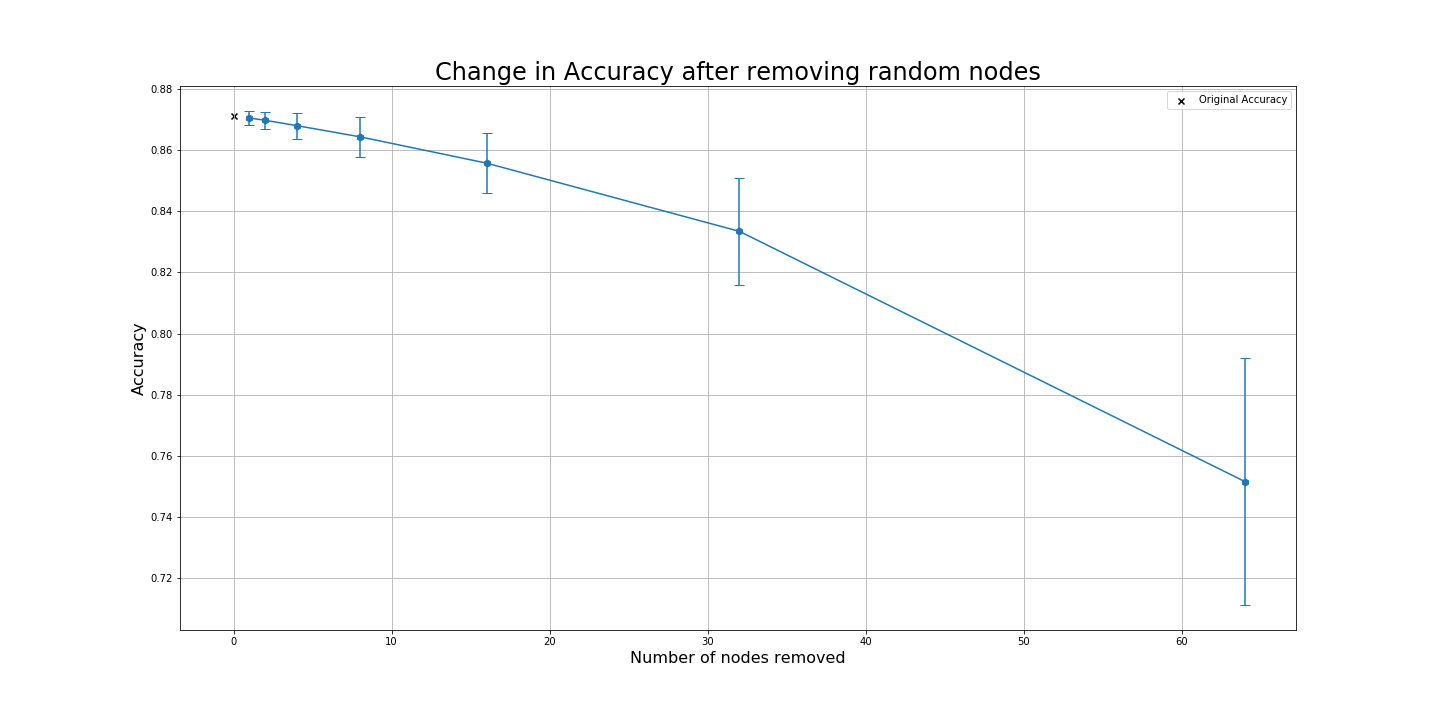
\includegraphics[width=\textwidth]{Accuracy_change_random_removal_fmnist.png}
                \caption[Short title]{Testing}
                \label{fig:acc_rn_fmnist}
            \end{figure}

            Trial text

            \begin{table}[h!]
                \centering
                \begin{tabular}{c | c c c c c c c}
                    & \multicolumn{7}{c}{\textbf{Number of Nodes}} \\
                    \cline{2-8}
                    & 1 & 2 & 4 & 8 & 16 & 32 & 64 \\
                    \hline
                    \textbf{Mean} & 0.9765 & 0.9760 & 0.9750 & 0.9724 & 0.9658 & 0.9464 & 0.8555 \\
                    \textbf{$\sigma$} & 0.0007 & 0.0010 & 0.0015 & 0.0027 & 0.0053 & 0.0122 & 0.0394 \\
                    \textbf{min} & 0.9740 & 0.9660 & 0.9635 & 0.9494 & 0.9337 & 0.8688 & 0.6598 \\
                    \textbf{25\%} & 0.9762 & 0.9756 & 0.9742 & 0.9710 & 0.9632 & 0.9410 & 0.8331 \\
                    \textbf{50\%} & 0.9767 & 0.9762 & 0.9753 & 0.9728 & 0.9669 & 0.9489 & 0.8616 \\
                    \textbf{75\%} & 0.9770 & 0.9767 & 0.9760 & 0.9742 & 0.9695 & 0.9543 & 0.8837 \\
                    \textbf{max} & 0.9778 & 0.9780 & 0.9779 & 0.9769 & 0.9769 & 0.9685 & 0.9334 \\
                    
                \end{tabular}
                \caption[Short]{Long}
            \end{table}

            Trial text

            \begin{figure}[h!]\centering
                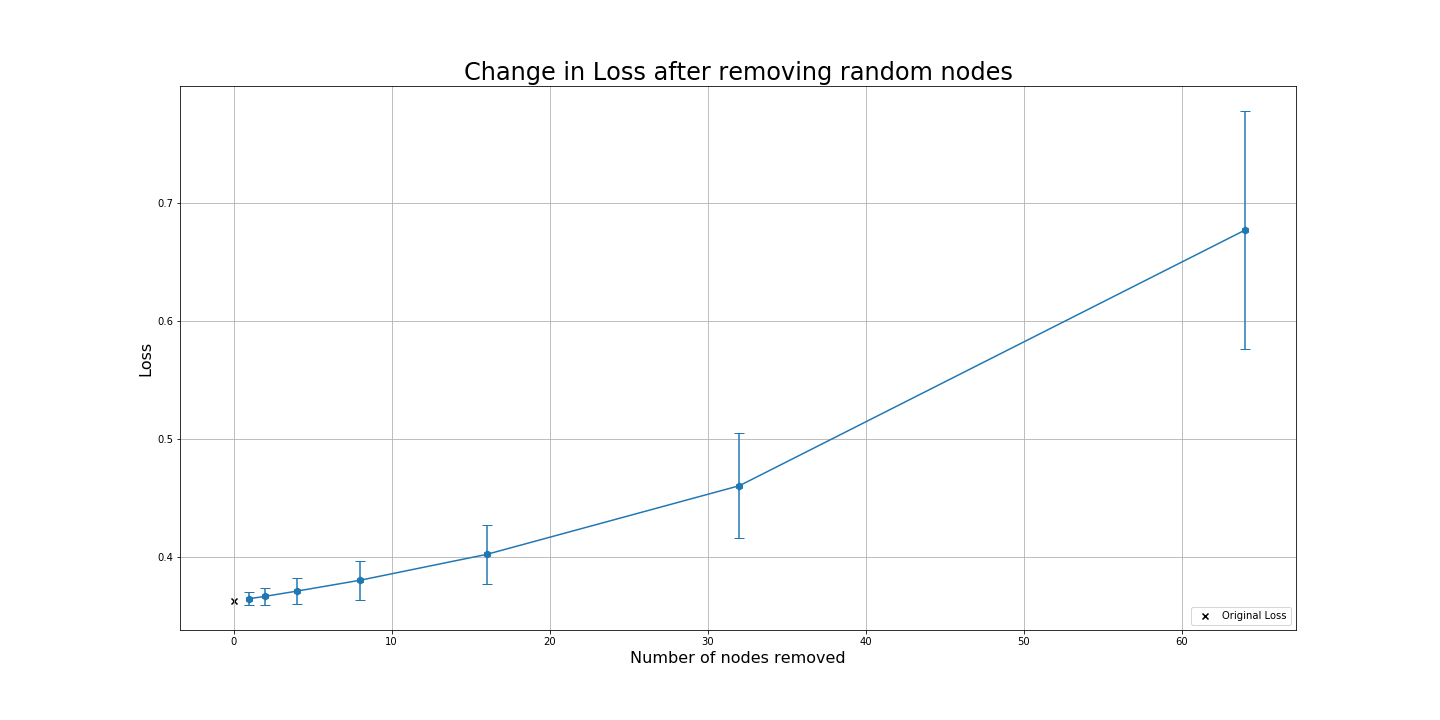
\includegraphics[width=\textwidth]{Loss_change_random_removal_fmnist.png}
                \caption[Short title]{Testing}
                \label{fig:loss_rn_fmnist}
            \end{figure}

            There is trial text here

            \begin{table}[h!]
                \centering
                \begin{tabular}{c | c c c c c c c}
                    & \multicolumn{7}{c}{\textbf{Number of Nodes}} \\
                    \cline{2-8}
                    & 1 & 2 & 4 & 8 & 16 & 32 & 64 \\
                    \hline
                    \textbf{Mean} & 0.0751 & 0.0767 & 0.0801 & 0.0885 & 0.1090 & 0.1680 & 0.4298 \\
                    \textbf{$\sigma$} & 0.0023 & 0.0032 & 0.0047 & 0.0083 & 0.0157 & 0.0338 & 0.0989 \\
                    \textbf{min} & 0.0720 & 0.0714 & 0.0710 & 0.0735 & 0.0791 & 0.1006 & 0.2311 \\
                    \textbf{25\%} & 0. & 0.9756 & 0.9742 & 0.9710 & 0.9632 & 0.9410 & 0.8331 \\
                    \textbf{50\%} & 0.9767 & 0.9762 & 0.9753 & 0.9728 & 0.9669 & 0.9489 & 0.8616 \\
                    \textbf{75\%} & 0.9770 & 0.9767 & 0.9760 & 0.9742 & 0.9695 & 0.9543 & 0.8837 \\
                    \textbf{max} & 0.9778 & 0.9780 & 0.9779 & 0.9769 & 0.9769 & 0.9685 & 0.9334 \\
                    
                \end{tabular}
                \caption[Short]{Long}
            \end{table}

            Trial text

            \begin{figure}[h!]\centering
                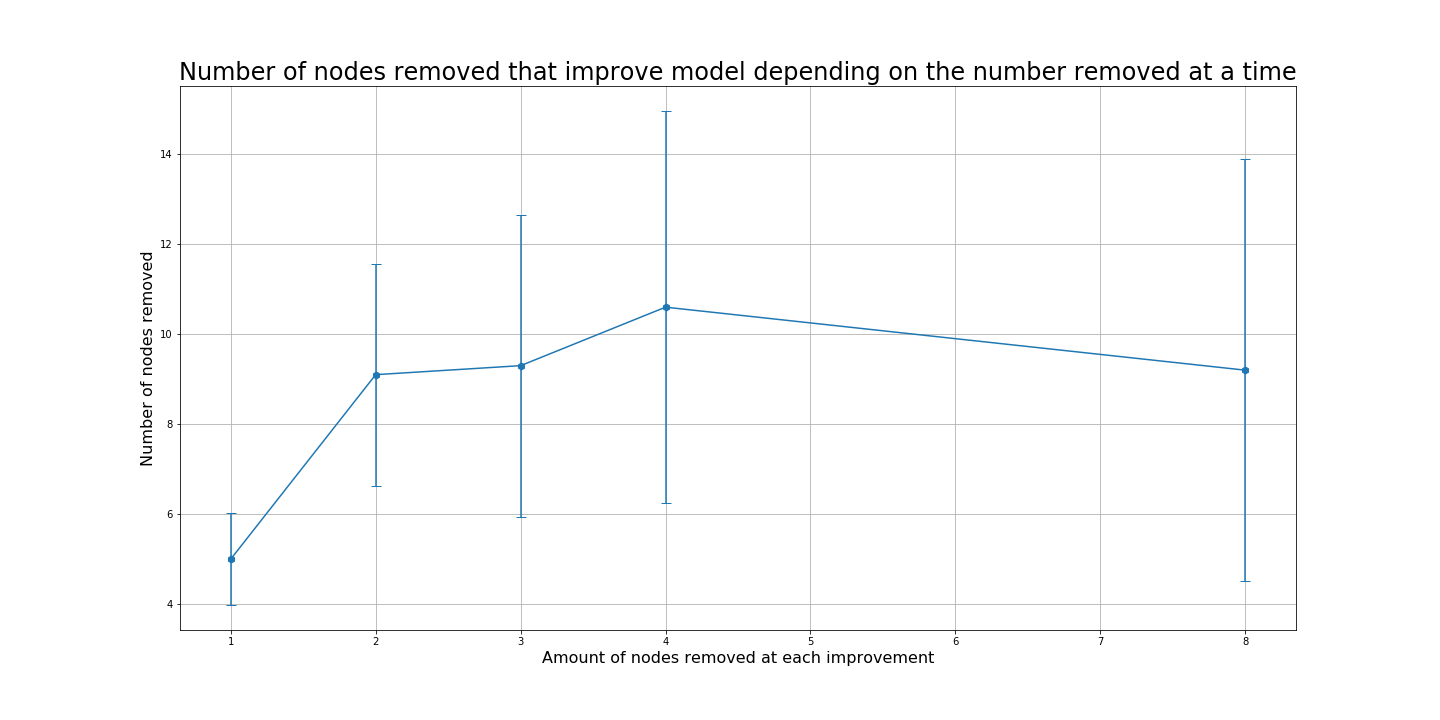
\includegraphics[width=\textwidth]{Num_rem_vs_size_removed_fmnist.png}
                \caption[Short title]{Testing}
                \label{fig:num_rem_rn_imp_fmnist}
            \end{figure}

            Trial text

            \begin{figure}[h!]\centering
                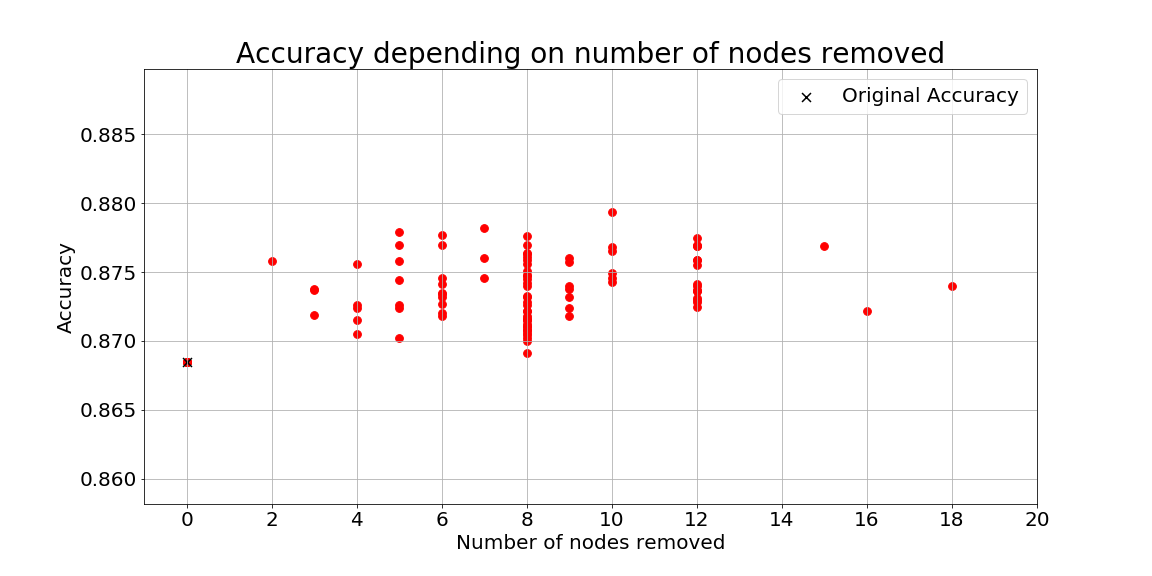
\includegraphics[width=\textwidth]{Accuracy_vs_nodes_removed_fmnist.png}
                \caption[Short title]{Testing}
                \label{fig:acc_rn_imp_fmnist}
            \end{figure}

            Trial text

            \begin{figure}[h!]\centering
                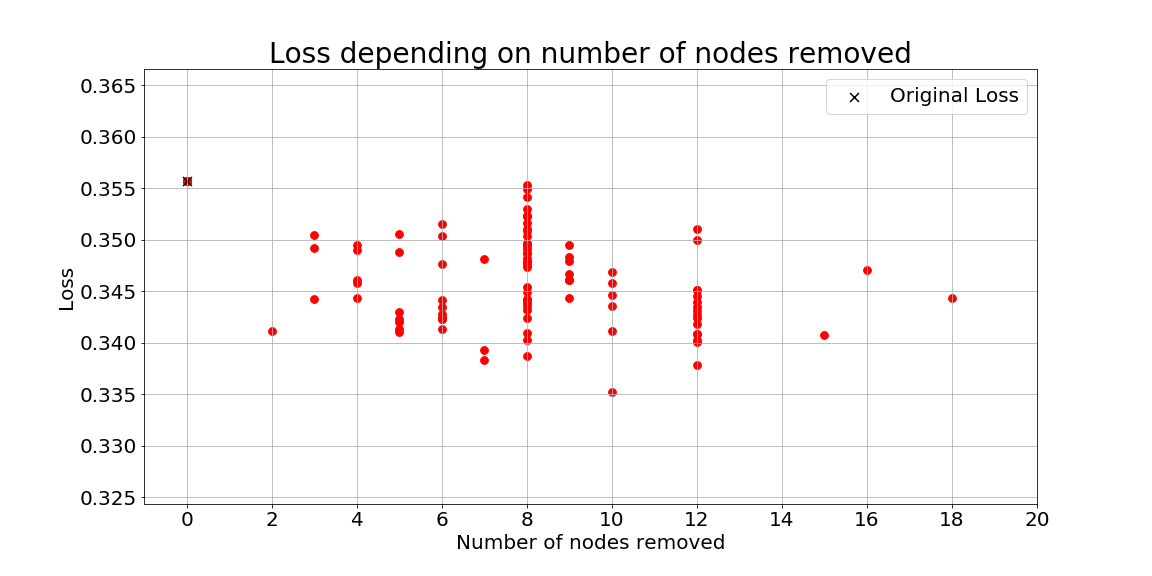
\includegraphics[width=\textwidth]{Loss_vs_nodes_removed_fmnist.png}
                \caption[Short title]{Testing}
                \label{fig:loss_rn_imp_fmnist}
            \end{figure}

            Trial text

    \section{Estimating Node Importance based on Loss and Accuracy}
    
    
    \section{Pruning Nodes based on the Loss and Accuracy}


    \section{Effects of Changing Training Batch Size on Node Importance}


    \section{Effects of Using Dropout}


\chapter{Multi-Layer Perceptron}
    \section{Pruning network with pre-calculated importance}


    \section{Greedy approach to pruning instead of Exhaustive approach}


    \section{Iterative weight initialization using Node importance}



\chapter{Convolutional Neural Network}
    \section{Looking at effects of per class accuracy after pruning}


    \section{Pruning based on class accuracy}


\chapter{Case study: Reducing a VGG-16 model trained on X dataset}

\chapter{Conclusion}
    \section{Summary}


    \section{Future Works}


\backmatter{}
\printbibliography
\end{document}